\documentclass[11pt, oneside]{amsart}   	% use "amsart" instead of "article" for AMSLaTeX format
\usepackage{geometry}                		% See geometry.pdf to learn the layout options. There are lots.
\geometry{letterpaper}                   		% ... or a4paper or a5paper or ... 
%\geometry{landscape}                		% Activate for rotated page geometry
%\usepackage[parfill]{parskip}    		% Activate to begin paragraphs with an empty line rather than an indent
\usepackage{graphicx}				% Use pdf, png, jpg, or eps§ with pdflatex; use eps in DVI mode
								% TeX will automatically convert eps --> pdf in pdflatex		
\usepackage{amssymb}
\usepackage{amsthm}
\usepackage{mathtools}
\usepackage{float}

\theoremstyle{definition}
\newtheorem{definition}{Definition}[section]
\newtheorem{theorem}{Theorem}[section]
\newtheorem{corollary}{Corollary}[theorem]
\newtheorem{lemma}[theorem]{Lemma}

\title{Math 250A Lecture Recaps (Modules)}
\author{Patrick Oare}
%\date{}							% Activate to display a given date or no date

\begin{document}
\maketitle

\section{10/3 (Free Modules, Projective Modules)}

\begin{itemize}

	\item A \textbf{module} over a ring $R$ is a set $M$ with a binary operation $+ : M\times M\rightarrow M$ and a map $\cdot: R\times M\rightarrow 
	M$ such that:
		
		\begin{enumerate}
		
			\item $(M, +)$ is an Abelian group.
			
			\item $(r_1r_2)m = r_1(r_2 m)$.
			
			\item $r(m_1 + m_2) = rm_1 + rm_2$.
			
			\item$ (r_1 + r_2)m = r_1m + r_2m$.
			
			\item $1m = m$ if $R$ has unity.
		
		\end{enumerate}
	
	\item \textbf{Homomorphisms of modules}: A map $f : M\rightarrow N$ is a homomorphism of $R-modules$ if $f(m + n) = f(m) + f(n)$ and $f(rm) = 
	rf(m)$. The better notation for this for left $R-modules$ is:
	$$
		mf := f(m)
	$$
	for it naturally suggests it commutes with ring elements, i.e. $(rm)f = r(mf)$. 
	
	\item \textbf{The $Hom$ functor}: Given 2 modules $M, N$ over $R$, the set of homomorphisms from $M$ into $N$, $Hom_R(M, N)$, forms an 
	abelian group under $+$. If $R$ is commutative, then $Hom_R(M, N)$ is itself a module over $R$ by defining $(rf)(m) := rf(m)$. Then, we see 
	that $Hom_R(\cdot, \cdot)$ is a bifunctor from $RMod$ to $Ab$ (or to $RMod$ if $R$ is commutative)-- $Hom_R(M, \cdot)$ is covariant, and 
	$Hom_R(\cdot, M)$ is contravariant. If we are dealing with vector spaces, then $Hom$ preserves exact sequences. This is not true in general. 
	Suppose:
	$$
		0\rightarrow A\xrightarrow{\phi} B\xrightarrow{\psi} C
	$$
	is exact. Then:
	$$
		0\rightarrow Hom(M, A)\xrightarrow{\phi'} Hom(M, B)\xrightarrow{\psi'} Hom(M, C)
	$$
	is also exact, where $\phi'(f) := \phi\circ f$. The first joint is easy, because if $f\in ker(\phi')$, $\phi\circ f = 0$. For any $m\in M$, $\phi(f(m)) = 0 
	\implies f(m) = 0$ as $\phi$ is injective by the exactness of the first diagram. Therefore, $\phi'$ has trivial kernel, so it is injective. To show that 
	$ker(\psi') = im(\phi')$ takes more work. Let $g\in ker(\psi')$, so $\psi\circ g = 0$. For $m\in M$, $\psi(g(m)) = 0$, so $g(m)\in ker(\psi) = im(\phi)$, 
	and thus $g(m) = \phi(a)$ for some $a$. $\phi$ is injective, so $a$ is uniquely specified given $m$, and thus the map $f: M\rightarrow A$, $f(m) := 
	a$ is well defined, and $f\in Hom_R(M, A)$. Then $\phi\circ f(m) = \phi(a) = g(m)$ by the definition, so $g = \phi\circ f$ and $ker(\psi')\subset 
	im(\phi')$. For the reverse containment, suppose $g\in im(\phi')$. Then $g = \phi\circ f$, so $\psi'(g) = \psi\circ g = \psi\circ\phi\circ f = \psi |im(\phi) 
	\circ\phi\circ f = 0$ as $\psi | im(\phi) = 0$, so $g\in ker(\phi')$, and the sequence is exact. For the converse, just use that $Hom_R(M, R)\cong M$.
	
	Similarly, if:
	$$
		A\rightarrow B\rightarrow C\rightarrow 0
	$$
	is exact, then:
	$$
		Hom(A, M)\leftarrow Hom(B, M)\leftarrow Hom(C, M)\leftarrow 0
	$$
	is exact. See the proof of this in Lang. $Hom_R$ preserves short exact sequences iff we are dealing with vector spaces or if the exact sequence 
	is \textbf{split}, so $B = A\oplus C$.
	
	We say that the $Hom$ functor is \textbf{left exact}, both when covariant and when contravariant.
	
	\item We also have the canonical isomorphism:
	$$
		Hom_R(R, M)\cong M
	$$
	for any R-module $M$, the isomorphism being given by $\phi\mapsto \phi(1)\in M$.
	
	\item For R-modules $A, B, C$, we have the following:
	$$
		Hom_R(A\oplus B, C)\cong Hom_R(A, C)\oplus Hom_R(B, C)
	$$
	and:
	$$
		Hom_R(A, B\times C)\cong Hom_R(A, B)\times Hom_R(A, C)
	$$
	where the isomorphisms are due to composing the homomorphisms with canonical injections and projections. To prove the first, let $\iota_A : A
	\rightarrow A\oplus B$, $\iota_B : B\rightarrow A\oplus B$ be the canonical inclusions. Let $f: A\oplus B\rightarrow C$, and define $\phi : Hom(A\oplus 
	B, C)\rightarrow Hom(A, C)\oplus Hom(B, C)$ by mapping:
	$$
		f\rightarrow (f\circ\iota_A, f\circ\iota_B)
	$$
	and this is an isomorphism.
	
	\item \textbf{Endomorphisms}: The set of \textbf{endomorphisms} of $M$ is $End(M) := Hom_R(M, M)$ forms a ring, where the product is 
	composition of endomorphisms. Then, we may view $M$ as a right module over $End(M)$, and the right action of $End(M)$ commutes with the 
	left action of $R$. We say that $M$ is a \textbf{$(R, End(M))$ bimodule}. If $R$ is commutative, then $M$ is an $End(M)$ module.
	
	\item \textbf{Representations}: Suppose $G$ is a group acting on a set $S$, and $K$ a field. We can turn $S$ into a vector space $V$ with basis 
	$S$ over $K$ by taking all $K$-linear combinations of $S$. Form the group ring $K[G]$, and then $V$ is a module over $K[G]$ by acting the 
	elements of $G$ on those of $S$. Suppose $M$ is a left module over $R$. 
	
	We may think of $End(M)$ as the permutations of $M$. Rings are often studied as a subring of $End(M)$ for some $T$-module M. For example, 
	consider $\mathbb Q[i]$. This is a vector space over $\mathbb Q$, and we think of elements of $\mathbb Q[i]$ as endomorphisms of the vector 
	space. Endomorphisms of a vector space are linear transformations, so we can represent the elements as matrices. We pick the basis $\{1, i\}$. 
	Then, $1$ sends $1$ to $1$ and $i$ to $i$, and $i$ sends $1$ to $i$ and $i$ to $-1$. Thus:
	$$
		1\longleftrightarrow 
		\begin{pmatrix}
			1 & 0 \\ 0 & 1
		\end{pmatrix}
		\;\;\;\;\;\;\;\;\;\;\;\;\;\;\;\;\;\;\;\;\;\;\;\;\;\;\;\;\;\;\;\;\;
		i\longleftrightarrow
		\begin{pmatrix}
			0 & -1 \\ 1 & 0
		\end{pmatrix}
	$$
	
	We can then think of $\mathbb Q[i]$ as matrices of the form:
	$$
		\begin{pmatrix}
			a & -b \\ b & a
		\end{pmatrix}
	$$
	with $a, b\in \mathbb Q$. These matrices have invariant properties under change of basis: trace and determinant. The trace is $2a$, and the 
	determinant is the norm $a^2 + b^2$ of the element.
	
	\item \textbf{Free modules}: A free module is a module that has a basis. If $M$ is a finitely generated free module over $R$, then:
	$$
		M \cong R \oplus R\oplus ... \oplus R
	$$
	
	We run into a problem: If $R^m\cong R^n$, does $m = n$?
		
		\begin{itemize}
			
			\item If $R$ is a field, this is true.
			
			\item If $R = 0$, then this is false.
			
			\item If $R$ is commutative and nonzero, this is true. Pick a maximal ideal $I\subset R$, and suppose $R^m = R^n$. Then we can 
			reduce this mod $I$, so $(R/I)^m \cong (R/I)^n$, which implies $m = n$ as $R / I$ is a field.
			
			\item Sometimes true if $R$ is not commutative. For example, we can take $R := M_{n \times n}(K)$. Then if $R^a = R^b$, we view 
			$R$ as a vector space over $K$ with dimension $n^2$, so this implies $an^2 = bn^2\implies a = b$. So in general, this holds if $R$ is a 
			vector space over a field.
			
			\item Ex of nontrivial ring where $R\cong \oplus R$ as $R$-modules: Pick an abelian group $A$ such that $A = A\oplus A$ (i.e. 
			$A = \oplus_{i = 1}^\infty\mathbb Z)$. Then, if we let $R = End(A)$, $R = Hom(A, A)\cong Hom(A, A\oplus A)\cong Hom(A, A) 
			\oplus Hom(A, A) \cong R\oplus R$.
			
		\end{itemize}
	
	Thus, the rank of a free module is not well defined as it is for vector spaces.
	
	\item \textbf{Adjoint Functors}: Let $F$ be the forgetful functor, $M$ an $R$-module, and $F(M) = S_M$. Let $F'$ be the functor taking a set $S$ 
	to the free module on $S$. Then given a set $S_N$, we form the free module $N := F'(S_N)$, and we have a commutative square for any 
	R-module homomorphism $f: M\rightarrow N$. We say that $F$ and $F'$ are \textbf{adjoint}: the map from the free module $M$ with basis $S_M
	$ to $N$ is the same as the map from $S_M$ to $S_N$. 
	
	\item \textbf{Sections}: Let 
	$$
		0\rightarrow A\xrightarrow{f} B\xrightarrow{g} C\rightarrow 0
	$$
	be an exact sequence of R-modules. We say the sequence \textbf{splits} if $B\cong A\oplus C$. A \textbf{section} is a map $\phi : C\rightarrow B$ 
	such that $g\circ\phi = id$, or a map $\psi : B\rightarrow A$ such that $\psi\circ f = id$. If such a section exists on one side, another exists on the 
	other side. If a section exists, then the sequence is split, so:
	$$
		B\cong im(f)\oplus ker(\psi) \cong ker(g)\oplus im(\phi)\cong A\oplus C
	$$
	
	\item \textbf{Projective Modules}: Let $P$ be an R-module. We say that $P$ is \textbf{projective} if it has the following property: If 
	$$
		M\rightarrow N\rightarrow 0
	$$
	is an exact sequence, (i.e. the homomorphism from $M$ to $N$ is surjective), then any map from $P\rightarrow N$ lifts to a map from $P
	\rightarrow M$ making the diagram commute.
	
	\item Free modules are projective.
	
	For suppose $F$ is free with basis $S$, and that $M\rightarrow N\rightarrow 0$ is exact. If we have a map $F\rightarrow N$, this induces a set 
	map $S\rightarrow N$. The map from $M$ to $N$ is surjective, so we can lift this set map to another map $S\rightarrow M$ giving a commutative 
	diagram. This induces a unique R-module homomorphism from $F$ to $M$ by the universal property which makes the diagram commute, and this 
	is the desired lift.
	
	\item \textbf{Theorem}: TFAE
	
		\begin{enumerate}
		
			\item P is projective.
			
			\item $P\oplus Q$ is free for some module $Q$.
			
			\item Every exact sequence 
			$$
				0\rightarrow N\rightarrow M\rightarrow P\rightarrow 0
			$$
			is split.
			
			\item The functor $Hom_R(P, \cdot)$ is exact.
		
		\end{enumerate}
	
	We show $P$ is projective iff $P\oplus Q$ is free for some module $Q$. Suppose $P$ is projective. Let $F$ be a free module equipped with a 
	surjective homomorphism $f:F\rightarrow P$ (we can pick $F = P$, so such a module exists). Then:
	$$
		F\xrightarrow{g} P\rightarrow 0
	$$
	is exact, and $P$ admits an identity isomorphism $P\xrightarrow{id} P$, so this identity lifts to $P\xrightarrow{\phi} F$. Such a $\phi$ is a section, as 
	$id = g\circ\phi$, so $F\cong im(\phi)\oplus ker(g)\cong P\oplus ker(g)$ as $\phi$ is an embedding. Suppose the converse, so $P\oplus Q$ is 
	free. $P\oplus Q$ is free, so $P\oplus Q$ is projective. Suppose $B\xrightarrow{g} C\rightarrow 0$ is exact, and we have a homomorphism $P
	\xrightarrow{\psi} C$. Let $\pi : P\oplus Q\rightarrow P$ be the canonical projection. Then we have a homomorphism $\psi\circ\pi$ from $P\oplus Q$ 
	into $C$, so this homomorphism lifts to $\Phi : P\oplus Q\rightarrow B$. The restriction $\phi := \Phi | P$ is then a lift of $\psi$, so $P$ is projective.
	
	\item We can visualize projective modules as "twisted" free modules; the Mobius band is an example of this. One way to show a module is projective 
	is to show that it is a summand of a free module, so if we have a surjective homomorphism $F\xrightarrow{g} M\rightarrow 0$ and we can find a 
	section $\phi : M\rightarrow F$ with $g\circ\phi = id$, then $M$ is projective.
	
	\item Example: take $R := \mathbb Z[\sqrt{-5}]$, and let $M := (2, 1 + \sqrt{-5})$. We show that $M$ is projective by showing that $M$ is a direct 
	summand of $R\oplus R$. We have an epimorphism $g : R\oplus R\rightarrow M$ given by:
	$$
		(1, 0)\mapsto 2\;\;\;\;\;\;\;\;\;\;\;\;\;\;\;\;\;\;\;\;\;\;\;\;\;\;\;\;\;\;\;\;\;\;\;\;\;(0, 1)\mapsto 1 + \sqrt{-5}
	$$
	A section of this map is given by $\phi: M\rightarrow R\oplus R$,
	$$
		\phi(m) := (-m, \frac{1 - \sqrt{-5}}{2}m)
	$$
	Then it can be verified that $g\circ\phi = id$, so $R\oplus R\cong M\oplus ker(g)$, and thus $M$ is a projective module.

\end{itemize}

\section{10/5 (Tensor Products)}

We let $R$ be a commutative ring, and $M, N$ be R-modules.

\begin{itemize}

	\item \textbf{Eilenburg-Mazur Swindle}: TODO 

	\item \textbf{Tensor Products}: We can view the tensor product of $M$ and $N$, $M\otimes N$, as a universal module in which every bilinear map 
	from $M\times N$ factors through. We have a R-bilinear map:
	$$
		\iota : M\times N\rightarrow M\otimes N
	$$
	such that given any R-bilinear map into an R-module $A$,
	$$
		\phi : M\times N\rightarrow A
	$$
	this map factors through the tensor product, i.e. there exists a unique R-module homomorphism $\Phi : M\otimes N\rightarrow A$ such that:
	$$
		\phi = \Phi\circ\iota
	$$
	
	\item \textbf{Construction of $M\otimes N$}: The tensor product is the quotient of the free module $F(M, N)$ by the submodule $H$ generated by 
	elements of the form $(m_1 + m_2, n) - (m_1, n) - (m_2, n)$, $(m, n_1 + n_2) - (m, n_1) - (m, n_2)$, $(rm, n) - r(m, n)$, and so on:
	$$
		M\otimes N := F(M, N) / H
	$$
	
	\item \textbf{Properties}: Here are some important properties, as well as ways to show them / think about them.
	
		\begin{enumerate}
		
			\item Distribution over the direct sum:
			$$
				(M_1\oplus M_2)\otimes N\cong (M_1\otimes N)\oplus (M_2\otimes N)
			$$
			Show that the map $(M_1\oplus M_2)\times N\rightarrow (M_1\otimes N)\oplus (M_2\otimes N)$, $((m_1, m_2), n)\mapsto (m_1\otimes n, 
			m_2\otimes n)$ is R-billinear. This induces the homomorphism in one direction, we can induce one in the other direction by making maps 
			$M_1\times N\rightarrow (M_1\oplus M_2)\otimes N$, $M_2\times N\rightarrow (M_1\oplus M_2)\otimes N$, factoring through the tensor 
			product, then joining them into a map from the direct sum. These maps are inverses.
			
			\item Tensor product with $R$:
			$$
				R\otimes M\cong M
			$$
			This is equivalent to saying the set of all bilinear maps out of $R\times M$ is in bijection with the set of R-linear maps out of $M$. To prove 
			this, show that $\phi : R\times M\rightarrow M$, $(r, m)\mapsto rm$ is R-bilinear, which induces the homomorphism $\Phi: R\otimes M
			\rightarrow M$, $r\otimes m\mapsto rm$. The inverse of this is $\theta : M\rightarrow R\otimes M$, $m\mapsto 1\otimes m$.
			
			\item Free modules:
			$$
				R^m\otimes R^n\cong R^{mn}
			$$
			To see this, induct on $n$ and use that $R^m\otimes R\cong R^m$. This generalizes for an arbitrary R-module $M$:
			$$
				R^n\otimes M\cong M^n
			$$
			This is simply the result of $R^n\otimes M\cong (\oplus_{i = 1}^n R)\otimes M\cong \oplus_{i = 1}^n (R\otimes M)\cong \oplus_{i = 1}^n M
			= M^n$.
			
			\item Associativity:
			$$
				(A\otimes B)\otimes C\cong A\otimes (B\otimes C)
			$$
			We can see this intuitively because trilinear maps shouldn't have a preference over their 3 domains. More rigorously, we can construct 
			inverse homomorphisms to one another. For $c\in C$, the map $\phi_c : A\times B\rightarrow A\otimes (B\otimes C)$, $(a, b)\mapsto 
			a\otimes (b\otimes c)$ is R-bilinear, and induces $\Phi_c : A\otimes B\rightarrow A\otimes (B\otimes C)$, $a\otimes b\mapsto a\otimes 
			(b\otimes c)$. We can then define $\phi : (A\otimes B)\times C\rightarrow A\otimes (B\otimes C)$, $(a\otimes b, c)\mapsto \Phi_c(a
			\otimes b) = a\otimes (b\otimes c)$, which is bilinear (obvious in the tensor, but can show for $c$). This induces $\Phi : (A\otimes B)
			\otimes C\rightarrow A\otimes (B\otimes C)$, $(a\otimes b)\otimes c\mapsto a\otimes (b\otimes c)$. We can find the inverse doing this 
			in the opposite way.
			
			\item Commutativity: 
			$$
				M\otimes N\cong N\otimes M
			$$
			
			Use the canonical map $\phi : M\times N\rightarrow N\otimes M$, $(m, n)\mapsto n\otimes n$. This is bilinear and induces $\Phi : M 
			\otimes N\rightarrow N\otimes M$, $m\otimes n\mapsto n\otimes m$. You can then find an inverse map $\Theta$ the other way, showing 
			these are isomorphic.
			
			\item $V\otimes W$ for K-vector spaces: As vector spaces are free modules, suppose $V\cong K^n$, $W\cong K^m$. Then $V\otimes W
			\cong K^{mn}$, and if $\{x_i\}_{i = 1}^n$ and $\{y_j\}_{j = 1}^m$ are bases for $V$ and $W$, respectively, then:
			$$
				\{x_i\otimes y_j\}_{i = 1, j = 1}^{n, m}
			$$
			is a basis for $V\otimes W$.
		
		\end{enumerate}
	
	\item \textbf{Left Adjoint Functors}: Let $C, D$ be categories. A functor $F: C\rightarrow D$ is \textbf{left adjoint} to a functor $G: D\rightarrow C$ if 
	the sets $Hom_C(F(X), Y)$ and $Hom_D(X, G(Y))$ are in bijection for all $X\in Obj(C), Y\in Obj(D)$.
	
	For the tensor product, we note that $Hom(A\otimes B, C)$ is the same as the set of bilinear maps from $A\times B$ to $C$, which is equivalent to 
	the set of linear maps $A\rightarrow Hom(B, C)$. So, the functor tensoring with $B$ is related to the functor $Hom_R(B, \cdot)$. The functor 
	$A\mapsto A\otimes B$ is left adjoint to the functor $C\rightarrow Hom_R(B, C)$. There is a simple analog to this; the functions from $R\times S$ to 
	$T$ are the same as the functions from $R$ to $Map(S, T)$. In the same way, the bilinear maps from $A\times B$ into $C$ are the same as the linear 
	maps from $A$ into $Hom_R(B, C)$. We have the bijection $Bil(A\times B, C)$ with $Hom_R(A, Hom_R(B, C))$ by sending:
	$$
		f(a, b)\in C\mapsto f(a, \cdot) : B\rightarrow C
	$$
	$$
		F(a) : B\rightarrow C\mapsto f(a, b) := f(a)(b)\in C
	$$
	So, in effect we can think of $Hom(A\otimes B, C)$ as either the set of bilinear maps $A\times B\rightarrow C$ or the set $Hom_R(A, Hom_R(B, C))$.
	
	\item \textbf{Right Exactness}: Suppose 
	$$
		A\rightarrow B\rightarrow C\rightarrow 0
	$$
	is exact. Then, for any module $M$:
	$$
		A\otimes M\rightarrow B\otimes M\rightarrow C\otimes M\rightarrow 0 
	$$
	is exact. We say that the functor $F(A) := A\otimes M$ is \textbf{right exact}, i.e. it preserves the right side of exact sequences.
	
	We can show this by recalling that $Hom(\cdot, M)$ is left exact, so given an exact sequence $A\rightarrow B\rightarrow C\rightarrow 0$, we have an 
	exact sequence
	$$
		Hom(A, M)\leftarrow Hom(B, M)\leftarrow Hom(C, M)\leftarrow 0
	$$
	
	Now, saying $A\otimes N\rightarrow B\otimes N\rightarrow C\otimes N\rightarrow 0$ is exact is equivalent to saying that $Hom(A\otimes N, M)
	\leftarrow Hom(B\otimes N, M)\leftarrow Hom(C\otimes N, M)\leftarrow 0$ is exact for all $M$. But by the discussion about left adjointness, this 
	is equivalent to the sequence $Hom(A, Hom(N, M))\leftarrow Hom(B, Hom(N, M))\leftarrow Hom(C, Hom(N, M))\leftarrow 0$ being exact. We see 
	that this is exact because the functor $Hom(\cdot, Hom(N, M))$ is left exact.
	
	The conclusion is that the functor $A\mapsto A\otimes M$ is right exact because the functor $Hom(\cdot, N)$ is left exact for all $N$. 
	
	\item \textbf{Calculating $M\otimes N$}: We can use the right exactness of $A\mapsto A\otimes M$ to calculate a presentation for $M\otimes N$. The 
	idea is to find an exact sequence of free R-modules:
	$$
		R^a\rightarrow R^b\rightarrow M\rightarrow 0
	$$
	Where $R^b$ will be seen as a set of generators and $R^a$ as a set of relations for the kernel of $R^b\rightarrow M$. We tensor with $N$:
	$$
		R^a\otimes N\rightarrow R^b\otimes N\rightarrow M\otimes N\rightarrow 0
	$$
	which gives us an exact sequence. We collapse this, as $R^n\otimes N\cong N^n$, giving the exact sequence:
	$$
		N^a\rightarrow N^b\rightarrow M\otimes N\rightarrow 0
	$$
	giving us a canonical isomorphism:
	$$
		M\otimes N\rightarrow N^b / im(N^a\rightarrow N^b)
	$$
	
	\item \textbf{$\otimes$ for Finitely Generated Abelian Groups}: As any finitely gen. abelian group is a direct sum of copies of $\mathbb Z$ and 
	$\mathbb Z / n\mathbb Z$ and $\otimes$ distributes over $\oplus$, it is enough to work out the tensor products of these as $\mathbb Z$-modules. 
	The first 3 cases are trivial:
	$$
		\mathbb Z\otimes \mathbb Z\cong \mathbb Z \;\;\;\;\;\;\;\;\;\;\;\;\;\;\; \mathbb Z\otimes \mathbb Z / n\mathbb Z\cong \mathbb Z / n \mathbb Z \;\;\;\;\;
		\;\;\;\;\;\;\;\;\;\; \mathbb Z / n\mathbb Z\otimes\mathbb Z\cong\mathbb Z / n \mathbb Z
	$$
	The last case is harder, so we wish to calculate $\mathbb Z / m\mathbb Z\otimes \mathbb Z / n\mathbb Z$. Take the exact sequence:
	$$
		\mathbb Z\xrightarrow{\times m}\mathbb Z\xrightarrow{\pi} \mathbb Z / m\mathbb Z\rightarrow 0
	$$
	Tensor this with $\mathbb Z / n\mathbb Z$ and collapse the tensors with $\mathbb Z$, giving:
	$$
		\mathbb Z / n\mathbb Z\xrightarrow{\times m}\mathbb Z/n\mathbb Z\rightarrow (\mathbb Z / m\mathbb Z)\otimes (\mathbb Z / n\mathbb Z)
		\rightarrow 0
	$$
	Now, we see that, since $im(\mathbb Z / n\mathbb Z\xrightarrow{\times m}\mathbb Z/n\mathbb Z) \cong m(\mathbb Z / n\mathbb Z)$:
	$$
		(\mathbb Z / m\mathbb Z)\otimes (\mathbb Z / n\mathbb Z)\cong \frac{\mathbb Z / n\mathbb Z}{m\mathbb Z / n\mathbb Z}\cong \mathbb Z / 
		\gcd(m, n)\mathbb Z
	$$
	
	\item Tensor products are not left exact. Consider the exact sequence:
	$$
		0\rightarrow \mathbb Z \xrightarrow{\times 2}\mathbb Z\rightarrow \mathbb Z / 2\mathbb Z\rightarrow 0
	$$
	After tensoring with $\mathbb Z / 2\mathbb Z$, we have:
	$$
		0\rightarrow\mathbb Z / 2\mathbb Z\xrightarrow{\times 2}\mathbb Z / 2\mathbb Z\rightarrow \mathbb Z / 2\mathbb Z\rightarrow 0
	$$
	which is not exact.
	
	\item \textbf{Tensor Products as Pushouts}: The tensor product is the pushout in the category of R-algebras, where $R$ is commutative. TODO
	
	\item Example: $\mathbb C \otimes_{\mathbb R}\mathbb C$. $\mathbb C$ has a basis $\{1, i\}$, so $\mathbb C\otimes \mathbb C$ has a basis 
	 $\{1\otimes 1, 1\otimes i, i\otimes 1, i\otimes i\}$. We note $(i\otimes i)(i\otimes i) = -1\otimes -1 = (-1)(-1)1\otimes 1 = 1\otimes 1$. Using this, can 
	 show:
	 $$
	 	e := \frac{1\otimes 1 + i\otimes i}{2}
	 $$
	 is an idempotent. Thus, $\mathbb C\otimes \mathbb C$ (as a ring) splits as a product $e(\mathbb C\otimes\mathbb C)\times (1 - e)\mathbb C\otimes 
	 \mathbb C\cong \mathbb C\times \mathbb C$, so:
	 $$
	 	\mathbb C\otimes_{\mathbb R}\mathbb C\cong \mathbb C\times\mathbb C
	 $$
	 as a ring.
	 
	 \item \textbf{K-Theory}: TODO
	 
	 \item \textbf{!!! Warnings about non-commutative rings !!!}: 
	 
	 	\begin{enumerate}
		
			\item $M\otimes_R N$ is only defined when $M$ is a right module and $N$ is a left module.
			
			\item $M\otimes_R N$ will only be an abelian group, not a module.
		
		\end{enumerate}
	
\end{itemize}

\section{10/10 (Duality, Colimits)}

\begin{itemize}

	\item \textbf{Dual Modules}: To create the dual in a category, we need a \textbf{dualizing object}. For modules (vector spaces), this is the 
	base ring (base field):
	$$
		M^* := Hom_R(M, R)
	$$
	$$
		V^* := Hom_K(V, K)
	$$
	
	If $M = R^n$, there is a natural isomorphism $M\rightarrow M^{**}$ by taking $m\mapsto f_m\in Hom_R(M^*, R)$, where $f_m:M^*\rightarrow R$, 
	$f_m(x) := x(m)$. It is also true that $M\cong M^*$, but the isomorphism is not natural; you need to pick a basis. This also holds for a projective $M$, 
	as then $M\oplus N$ is free and has this property. Note that:
	$$
		(M\oplus N)^*\cong M^*\oplus N^*
	$$
	as $Hom_R(M\oplus N, R)\cong Hom_R(M, R)\oplus Hom_R(N, R)$.
	
	\item \textbf{Dual Groups}: We pick the dualizing object for groups to be $\mathbb Q / \mathbb Z\cong S^1$, where $S^1 = \mathbb C^*$ is the circle 
	group. We have:
	$$
		G^* := Hom(G, \mathbb Q / \mathbb Z)
	$$
	Note that $Hom(G, \mathbb Q / \mathbb Z) = Hom(G, \mathbb Z / n\mathbb Z)$, where $n = |G|$. We also have $G\cong G^*$-- we show this 
	property for cyclic groups, then use that finitely generated abelian groups are direct sums of these. This is because $Hom(\mathbb Z / n\mathbb Z, 
	\mathbb Q / \mathbb Z) = \{$elements of order $n$ in $\mathbb Q / \mathbb Z$ $\} = \{0, \frac{1}{n}, \frac{2}{n}\} = \langle\frac{1}{n}\rangle\cong 
	\mathbb Z / n\mathbb Z$. This isomorphism is \textbf{not natural}-- it depends on explicitly where you send the generator to.
	
	\item \textbf{Dirichlet Characters}: A Dirichlet character $\chi$ mod $N$ is an element of the dual of $(\mathbb Z / N\mathbb Z)^\times$ (will use $F^
	\times$ for multiplicative group of a ring to avoid confusion). For example, the characters for $N = 8$ are ($\phi(8) = 4$, so expect $4$ characters):
	
	\begin{table}[H]
		\centering
		\begin{tabular}{| c | c | c | c | c |}
			\hline
			$(\mathbb Z / 8\mathbb Z)^\times$ & 1 & 3 & 5 & 7 \\
			\hline
			$\chi_0$ & 1 & 1 & 1 & 1 \\
			\hline
			$\chi_1$ & 1 & -1 & 1 & -1 \\
			\hline
		\end{tabular}
		\caption{Dirichlet Characters for $N = 8$}
	\end{table}
	
	Note that $\chi$ is determined by its value on $3$ and $5$ as $7 \equiv 3\times 5\mod 8$, so $3$ and $5$ generate the group. Furthermore, every 
	element has order 2 so must be sent to $\pm 1$. We can define the \textbf{Dirichlet L Function} for a given character $\chi$:
	$$
		L(s, \chi) := \sum_{n = 1}^\infty\frac{\chi(n)}{n^s}
	$$
	
	\item \textbf{Orthogonality}: The Dirichlet characters are \textbf{orthogonal} in the following sense: Suppose $\chi_1\neq\chi_2$ are Dirichlet 
	characters mod $N$. We can define an inner product:
	$$
		(\chi_1, \chi_2) := \sum_{y\in(\mathbb Z / N\mathbb Z)^\times}\chi_1(y)\bar\chi_2(y)
	$$
	We can define $\chi := \chi_1\bar\chi_2$. We see $\chi = \chi_1\bar\chi_2\neq\chi_1\bar\chi_1 = 1$, and we wish to show $(\chi, 1)\neq 0$ as $(\chi, 
	1) = (\chi_1, \chi_2)$. Pick $a\in(\mathbb Z / N\mathbb Z)^\times$ with $\chi(a)\neq 1$. Then:
	$$
		\sum_{x\in(\mathbb Z / N\mathbb Z)^\times}\chi(x) = \sum_{y = a^{-1}x}\chi(ay) = \chi(a)\sum_{y\in(\mathbb Z / N\mathbb Z)^\times}\chi(y)
	$$
	as changing to $y$ just reindexes the sum over all $(\mathbb Z / N\mathbb Z)^\times$. As $\chi(a)\neq 1$, this implies:
	$$
		(\chi_1, \chi_2) = (\chi, 1) = \sum_{x\in(\mathbb Z / N\mathbb Z)^\times}\chi(x) = 0
	$$
	
	\item \textbf{Fourier Transform}: Let $G$ be a finite group, and $f : G\rightarrow \mathbb C$ a function. We define the Fourier Transform of $f$, 
	$\tilde f : G^*\rightarrow\mathbb C$ by:
	$$
		\tilde f(\chi) := (\chi, f) = \sum_{x\in G}\chi(x)\bar f(x)
	$$
	When we consider the dual of infinite abelian groups, the dualizing object is still $S^1$, the groups should be locally compact, and all 
	homomorphisms should be continuous. For example, the dual of $\mathbb Z$ is $\mathbb Z^* = Hom(\mathbb Z, S^1) = Hom_\mathbb Z(\mathbb Z, 
	S^1)\cong S^1$. Similarly, $(S^1)^* = Hom(S^1, S^1)$ is all continuous homomorphisms on $S^1$, which are of the form $z\mapsto z^n$ for $n\in 
	\mathbb Z$, so $(S^1)^*\cong\mathbb Z$, and thus $S^1$ and $\mathbb Z$ are dual to one another. For $G := \mathbb R$, $G^* = Hom(\mathbb R, 
	S^1)\cong\mathbb R$ by $x\mapsto exp(ixy) \in G^*$. So, the Fourier Transform takes a function on $G = \mathbb R$ to a function on $G^* = 
	\mathbb R$. 
	
	\item \textbf{Divisible Groups}: A group $G$ is \textbf{divisible} if $\forall g\in G, n\in\mathbb N$, $\exists h\in G$ such that $nh = g$. Essentially, we 
	can divide group elements by integers. The stereotypical example of a divisible group is $\mathbb Q$. Any product, direct sum, or quotient of a 
	divisible group is divisible, so $S^1\cong \mathbb Q / \mathbb Z$ is divisible. 
	
	\item \textbf{Injective Modules}: A module $I$ is \textbf{injective} if given any exact sequence:
	$$
		0\rightarrow B\xrightarrow{\phi} A
	$$
	and any homomorphism $B\xrightarrow{f} I$, there is a lift $A\xrightarrow{F} I$ such that $f = F\circ\phi$. Now, \textbf{any module divisible as an 
	abelian group is injective}.
	
	To show this, we consider $B$ as a submodule of $A$. Pick $a\in A\setminus B$. Pick the smallest $n\in\mathbb N$ such that $na\in B$, if such an 
	$n$ exists. Then, $x := f(na)\in I$, so we can divide it by $n$. Let $g\in I$ be this element with $x = ng$. Then, $ng = f(na)$, and we define $g := f(a)$ 
	to extend the homomorphism $f$ to $a$. If such an $n$ does not exist, set $f(a)$ to be any element of $I$. Now we can extend $f$ to $A$ with 
	Zorn's Lemma: TODO.
	
	\item Every abelian group is contained in an injective module. For given an abelian $G$ and $0\neq a\in G$, we can construct a homomorphism 
	$f: G\rightarrow \mathbb Q / \mathbb Z$ with $f(a)\neq 0$. We can concatenate copies of these homomorphisms for each $a\in G$, and view 
	$G$ as a subset of a (possibly infinite) number of copies of $\mathbb Q / \mathbb Z$. 
	
	\item For any ring $R$, the dual of $R$ as a $\mathbb Z$ module: 
	$$
		Hom_\mathbb{Z}(R, \mathbb Q / \mathbb Z)
	$$
	is an injective right R-module where we define $(fr)(s) := f(rs)$ for any $f\in Hom_{\mathbb Z}(R, \mathbb Q / \mathbb Z)$. The key point is:
	$$
		Hom_R(M, Hom_\mathbb{Z}(R, \mathbb Q / \mathbb Z))\cong Hom_\mathbb{Z}(M, \mathbb Q / \mathbb Z)
	$$
	which allows us to lift any map from $B\rightarrow R^*$, where $0\rightarrow B\rightarrow A$ is exact. 
	
	\item \textbf{Colimits}: Let $C$ be a category. A colimit of a family of objects $\{G_i\}_{i\in I}$ in $C$ is an object $G$ equipped with morphisms:
	$$
		f_i : G_i\rightarrow G
	$$
	making any composition of these morphisms commute, and with the universal property that any other object $H$ having this property has a unique 
	morphism $G\rightarrow H$ respecting all the arrows. Suppose that we have a sequence of objects and morphisms:
	$$
		G_0\xrightarrow{f_1} G_1 \xrightarrow{f_2} G_2\xrightarrow{f_3}...
	$$
	where each $f_i$ is injective. Then the colimit of this is their union:
	$$
		colim (G_i) = \bigcup_{i\in I}G_i
	$$
	equipped with the canonical inclusion maps for all $i$. A concrete example is the collection:
	$$
		\mathbb Z\rightarrow \frac{1}{2}\mathbb Z\rightarrow \frac{1}{6}\mathbb Z\rightarrow ...
	$$
	where each arrow is an embedding. Then, the colimit of this is $\mathbb Q = \cup_{n = 1}^\infty\frac{1}{n!}\mathbb Z$.
	
	\item \textbf{Colimits are right exact}: Suppose we have a collection of exact sequences:
	$$
		0\rightarrow A_i\rightarrow B_i\rightarrow C_i\rightarrow 0
	$$
	
	Where each of these are equipped with morphisms $A_i\rightarrow A_{i + 1}$. If we take the colimit of this sequence, then:
	$$
		colim (A_i)\rightarrow colim (B_i)\rightarrow colim(C_i)\rightarrow 0
	$$
	is also exact, so $colim$ is a right exact functor.
	
	\item \textbf{Direct Limits}: We say $I$ is a directed set if $I$ is a poset and $\forall i, j\in I$, there is some $k\in I$ such that $i\leq k, j\leq k$. Let  
	$\{M_i\}_{i\in I}$ be a system of objects in a category equipped with morphisms $f^i_j : M_i\rightarrow M_{j}$:
	$$
		M_1\xrightarrow{f^1_2} M_2\xrightarrow{f^2_3} M_3\xrightarrow{f^3_4} ...
	$$
	
	We define the \textbf{direct limit} of this family, $\varinjlim M_i$, to be the colimit of this directed sequence. The direct limit also has a morphism 
	into each object in the family:
	$$
		f^i : M_i\rightarrow \varinjlim M_i
	$$
	The direct limit is an \textbf{exact 
	functor}, i.e. it preserves exact sequences. For a proof, check the homework.
	
	\item \textbf{Inverse Limits}: The "dual" notion of a direct limit is an inverse limit. Suppose we have an inversely directed system:
	$$
		M_1\xleftarrow{f^2_1} M_2\xleftarrow{f^3_2} M_3\xleftarrow{f^4_3} ...
	$$
	Then the inverse limit is a a universal object with morphisms:
	$$
		f_i : \varprojlim M_i \rightarrow M_i
	$$
	The inverse limit is a left exact functor, so it does not preserve surjectivity of maps.
	
	\textbf{Direct Limits in RMod}: Let $M_1\rightarrow M_2\rightarrow ...$ be a directed sequence of R-modules. Intuitively, we can think of the direct 
	limit as their union quotiented by an equivalence relation. Two elements from different $M_i$'s are equal iff their images \textbf{eventually become 
	equal}. Mathematically, we let:
	$$
		B := \bigcup_{i\in I}M_i
	$$
	and define an equivalence relation for $(a, b)\in B\times B$ with $a\in M_i$ and $b\in M_j$:
	$$
		a\equiv b \iff \exists k\geq i, j : f^i_k(a) = f^j_k(b)
	$$
	The direct limit is then:
	$$
		\varinjlim M_i = B / \equiv
	$$
	equipped with the addition:
	$$
		\bar a + \bar b := \overline{f^i_k(a) + f^j_k(b)}
	$$
	which can be shown to be well defined. This equivalence relation makes it clear that elements are the same if and only if they eventuallly become 
	equal in the directed system of morphisms.

\end{itemize}

\section{10/12 (Snake Lemma, Mittag-Leffler Condition)}

\begin{itemize}

	\item \textbf{Snake Lemma}: The snake lemma says that we get a long exact sequence between the kernels and the cokernels of the following 
	diagram:
	
	\begin{figure}[H]
		\centering
		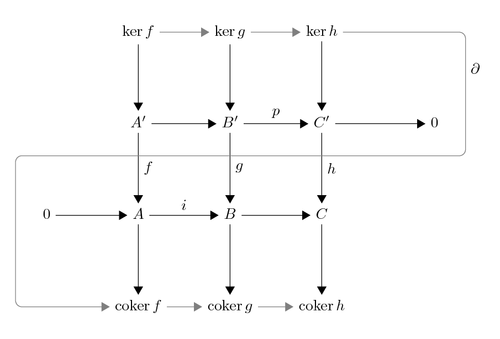
\includegraphics[width = .6\textwidth]{snake_lemma}
		\caption{Snake Lemma}
	\end{figure}
	
	To define the connecting map $\partial$, we "zigzag" around the diagram.
	
	\item \textbf{Tor Functor}: TODO.
	
	\item \textbf{Homology Groups}: TODO.
	
	\item \textbf{Mittag-Leffler Condition}: TODO.

\end{itemize}

\end{document}  